\section{Memory Faults}
\label{sect:bg-faults}
Precise fault modeling is the key to designing efficient fault tests.  Fault models reflect real, specific defects in memory so high defect coverage and detection is strongly dependent on the quality of the fault model \cite{1327984}.  The following sections offer a brief description about the four classic types of faults that models are designed to detect \cite{Adams2003}.  

\subsection{Stuck-At Faults}
The most common type of memory fault occurs when the memory cell state is locked into either a \textit{0} (SA0 fault) or \textit{1} (SA1 fault).  A defect-free cell can be written to either state and when read, will still contain the information previously written.  The stuck-at fault (SAF) occurs when a state is written to the cell, but the subsequent read returns only one state regardless of the previously written value.  Figure \ref{fig:sd-sa0f} and Figure \ref{fig:sd-sa1f} show the state diagrams for SA0 and SA1 faults.  Another fault that can be classified as a SAF is the address decoder fault.  It is similar to the data SAF, but occurs on the address lines.  It characteristics include accessing wrong addresses, no addresses or multiple addresses \cite{VanDeGoor1991}.
\begin{figure}[H]
  \centering
  \begin{subfigure}[b]{0.5\textwidth}
    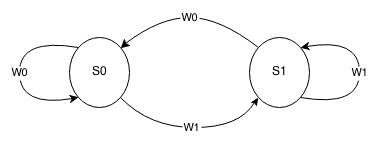
\includegraphics[width=\textwidth]{sd-gc}
    \caption{State diagram of a good cell}
    \label{fig:sd-gc}
  \end{subfigure}  
  
  \begin{subfigure}[b]{0.25\textwidth}
    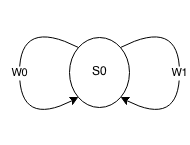
\includegraphics[width=\textwidth]{sd-sa0f}
    \caption{SA0 Fault}
    \label{fig:sd-sa0f}
  \end{subfigure}  
  \begin{subfigure}[b]{0.25\textwidth}
    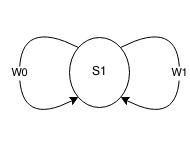
\includegraphics[width=\textwidth]{sd-sa1f}
    \caption{SA1 Fault}
    \label{fig:sd-sa1f}
  \end{subfigure}  
  
  \begin{subfigure}[b]{0.5\textwidth}
    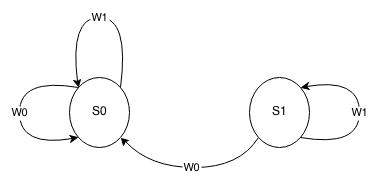
\includegraphics[width=\textwidth]{sd-tf}
    \caption{\textit{0\ding{221}1} Transition Fault}
    \label{fig:sd-tf}
  \end{subfigure}  

  \caption[State Diagrams for a Single Cell]{State Diagrams for a Single Cell \cite{VanDeGoor1991}}
  \label{fig:sd-sc}
\end{figure}

\subsection{Transition Faults}
Similar to a SAF, the transition fault (TF) also locks into a single state, but has the characteristic of being in either state prior to the write.  The memory cell may contain \textit{0} or \textit{1} when powered on, but after a write, it cannot transition back.  The characteristic behavior of this fault is the memory can only be written in one direction.  An example of a \textit{0\ding{221}1} TF is shown in Figure \ref{fig:sd-tf}.

\subsection{Coupling Faults}
There are numerous types of coupling faults (CF), but they can be simply expressed as a cell affecting its neighboring cells and causing the neighbor to falsely transition or change state \cite{VanDeGoor1991}.  Coupling faults can be unidirectional or bi-directional.  In unidirectional CF, one cell (the aggressor cell) couples to another cell (the victim cell), but the inverse does not occur \cite{Adams2003}.  A parasitic diode connection between the cells is a common cause of this behavior.  The bi-directional CF occurs when a pair of cells affect each other.  One way that this type of defect can occur is through bridging \cite{Adams2003}.  

\subsection{Neighborhood Pattern-Sensitive Fault (NPSF)}
\label{sec:npsf}
This fault model is in the class of CF, but rather than one specific aggressor cell, the coupling is caused by a particular pattern of values in neighboring cells.  The neighborhoods are usually defined as Type-1 or Type-2 neighborhoods \cite{1047051} as shown in Figure \ref{fig:npsftypes}.  Type-1 neighborhoods consist of five cells: one cell in center and four cells physically adjacent to the center cell.  In this configuration, the center cell is the base cell and the four adjacent cells are called the deleted neighborhood.  Type-2 neighborhoods consist of multiple cells where the base cell is in the center and deleted neighborhood is comprised of the cells within $m_1$ columns to the left, $m_2$ rows above, $m_3$ columns to the right and $m_4$ rows below the base cell \cite{VanDeGoor1991}.  This report will focus on Type-1 neighborhoods.

\begin{figure}[H]
  \centering
  \begin{subfigure}[b]{0.4\textwidth}
    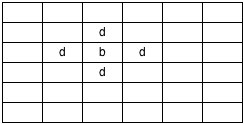
\includegraphics[width=\textwidth]{type1}
    \caption{Type-1 Neighborhood}
    \label{fig:type1}
  \end{subfigure}
  \begin{subfigure}[b]{0.4\textwidth}
    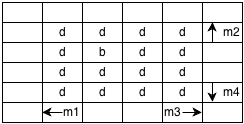
\includegraphics[width=\textwidth]{type2}
    \caption{Type-2 Neighborhood}
    \label{fig:type2}
  \end{subfigure}
  \caption[NPSF Neighborhoods]{NPSF Neighborhoods} 
           b: base cell \\
           d: deleted neighborhood \\
           b+d: neighborhood
           %$m_1$ = $m_2$ = 1; $m_3$ = $m_4$ = 2}
  \label{fig:npsftypes}
\end{figure}

Algorithms specify that the deleted neighborhood must be in the physical proximity of the base cell because only those cells are likely to influence the base cell.  Since the NPSF requires a specific pattern in memory which requires additional overhead, algorithms are written to detect all types of NPSF rather than a signle type.  Three classes of NPSF faults exist:
\begin{enumerate}
  \item Active NPSF (ANPSF) \cite{1675601}: the base cell's contents change due to changes in the pattern of the deleted neighborhood.
  \item Passive NPSF (PNPSF) \cite{1675601}: the base cell's contents cannot change due to specific pattern in the deleted neighborhood.
  \item Static NPSF (SNPSF) \cite{1676572}: the base cell's contents are forced to a specific value because of the contents of the deleted neighborhood
\end{enumerate}

To test for all three classes of NPSF, all the combinations of values in the deleted cells and their transitions must be performed against the base cell.  To do this, a Eulerian Sequence is employed to generate the appropriate sequence of values in the neighborhood.  The Eulerian Sequence has been proven to be an acceptable testing mechanism for NPSF \cite{1675556}.  A 5-bit Eulerian Sequence is used as the Type-1 patterns.

To reduce the number of write operations to memory, multiple patterns can be written to memory simultaneously using either the tiling or two-group methods as shown in Figures \ref{fig:type1tiling} and \ref{fig:type1group}.  With the tiling method, the memory is entirely written with a group of neighborhoods that do not overlap \cite{VanDeGoor1991}.  The two-group method takes advantage of the \textit{duality of cells}: a cell can simultaneously be the base cell in one group and part of the deleted neighborhood in a second group \cite{1675601}.  

\begin{figure}[H]
  \centering
  \begin{subfigure}[b]{0.4\textwidth}
    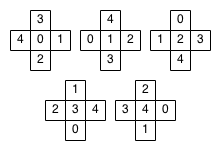
\includegraphics[width=\textwidth]{type1-tiling}
    \caption{Tile Groupings for 5-bit Patterns}
    \label{fig:type1-tl}
  \end{subfigure}
  \begin{subfigure}[b]{0.4\textwidth}
    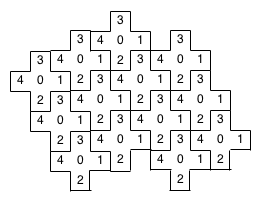
\includegraphics[width=\textwidth]{type1-tiling-neighborhood}
    \caption{Tiling Neighborhood with Base Cell 0}
    \label{fig:type1-tlnh}
  \end{subfigure}
  \caption[Type-1 Neighborhood Tiling Method]{Type-1 Neighborhood Tiling Method \cite{VanDeGoor1991}}
  \label{fig:type1tiling}
\end{figure}

\begin{figure}[H]
  \centering
  \begin{subfigure}[b]{0.4\textwidth}
    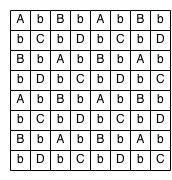
\includegraphics[width=\textwidth]{type1-tg1}
    \caption{Group 1 Cell Labels}
    \label{fig:type1-tg1}
  \end{subfigure}
  \begin{subfigure}[b]{0.4\textwidth}
    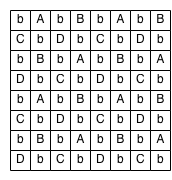
\includegraphics[width=\textwidth]{type1-tg2}
    \caption{Group 2 Cell Labels}
    \label{fig:type1-tg2}
  \end{subfigure}
  \caption[Type-1 Neighborhood Tiling and Two-Group Method]{Type-1 Neighborhood Tiling and Two-Group Method \cite{1675601},\cite{1676572}}
  \label{fig:type1group}
\end{figure}

In the tile groupings shown in Figure \ref{fig:type1-tl}, the center cell is considered the base cell.  Each of the bits in the 5-bit pattern will at some point during the test be positioned in the base cell.  Figure \ref{fig:type1-tlnh} illustrates how a tile with base cell \textit{0} could be written to memory in such a way that none of the tiles overlap.  The two cell groupings shown in Figures \ref{fig:type1-tg1} and \ref{fig:type1-tg2} demostrate how the two checkerboard patterns are overlaid in such a way that a cell can be a base cell is one checkerboard pattern while in the deleted neighborhood in the other checkerboard pattern.  This report will focus on the tiling method.
